% (C) Marc Lijour, 2018 
% Licensed under a Creative Commons License BY-SA
% https://creativecommons.org/licenses/by-sa/2.5/ca/
% Presentation at the BlockchainHub at York University
%       BlockChain and Intellectual Property
%       Toronto: August 9, 2018 at 6:30 pm
%	https://www.meetup.com/The-BlockchainHub-v0/events/250743088/
% authored by Marc Lijour, August 2018
% 
% Plan
% - pb stmt: 
% - EEA stack
% - Application in court: \cite{chinesecourt2018} % Baoquan.com compresses and packs screenshots, source code and invocation log, and stores the encryption hash value of the same on the Factom and Bitcoin blockchains. This leads the court to examine if blockchain technology as such is reliable, which it ultimately approves.
% Stories: (who is gaining/losing the most? whocan gain the most to improve on the status quo?)
% - RMS printer story
% - AI start up w secret sauce
% - Apple vs Samsung
% - ORACLE (java) vs Google
% - Elon Musk open source cars
% - 
% - 
% === What Blockchain brings to the picture
% -

% ======================================================================================================
%                                     Stories illustrating challenges with IP
% ======================================================================================================
\section{The good, the bad, and the ugly in Tech IP}
\frame{
	\frametitle{For Want of a Printer}
	\begin{figure}
		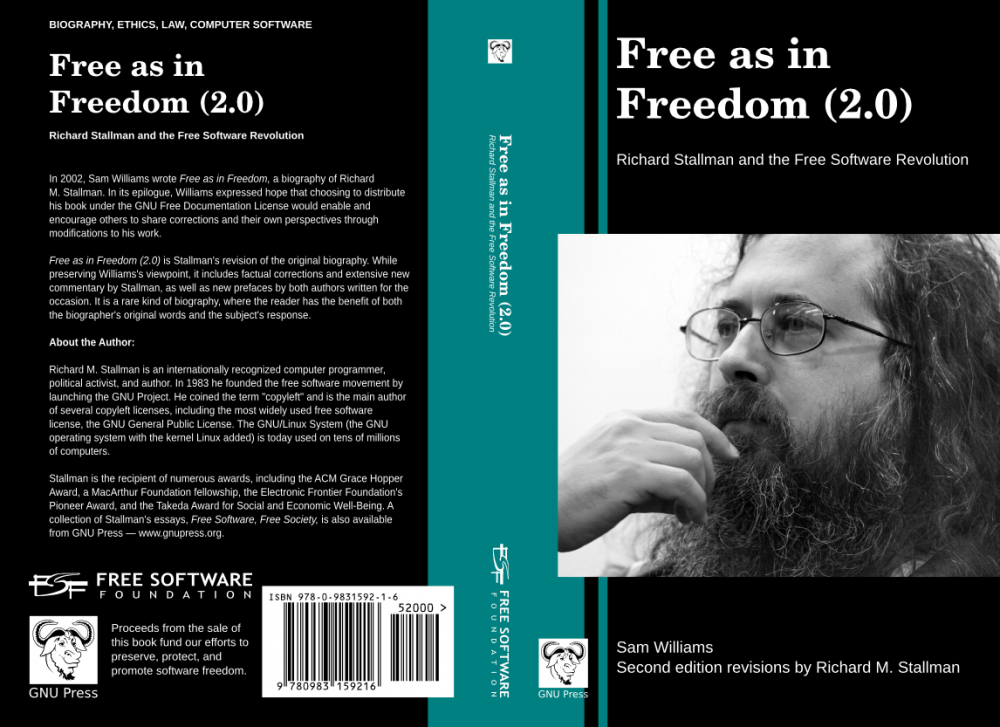
\includegraphics[height=6cm]{../pics/floss/productimage-picture-free-as-in-freedom-2-92}
		\caption{Richard Stallman's first step into Free Software (\cite{rms02:freedombook}; \cite{rms10:freedombook})}
	\end{figure}
}

\frame{
	\frametitle{Patents and the future of Intelligence}
	\begin{figure}
		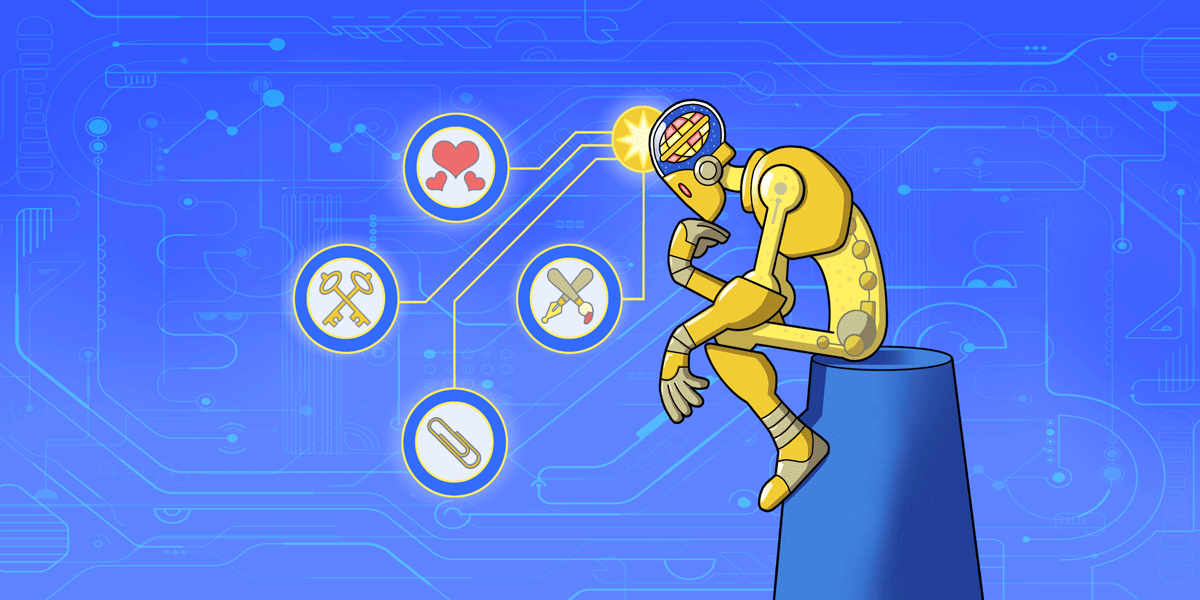
\includegraphics[width=11cm]{../pics/AI/eff-artificial-intelligence-ccby}
		\caption{The \citeauthor{eff17:ai} (EFF) questions whether patents will slow down innovations in AI (\citeyear{eff17:ai}) --credit: EFF}
	\end{figure}
}

\frame{
	\frametitle{What's (un)fair with APIs}
	\begin{itemize}
		\item \emph{Oracle America, Inc. v. Google, Inc.} took us for a ride (2012--2016), see \citeauthor{wikipedia:oraclevsjava}'s article in the reference section
		\item the US Court of Appeal for the Federal Circuit found that \textbf{APIs are copyrightable} (\citeyear{uscourtappealfedcirc18:oraclejava})
		\item \emph{fair use} does not apply for Java in Android
		\item in 2016 Google ships OpenJDK Java libraries licensed under GPLv2, starting with Android Nougat (\citeauthor{androidlicense})
	\end{itemize}
}

\frame{
	\frametitle{Elon Musk does not want to block Innovation}
	\begin{figure}
		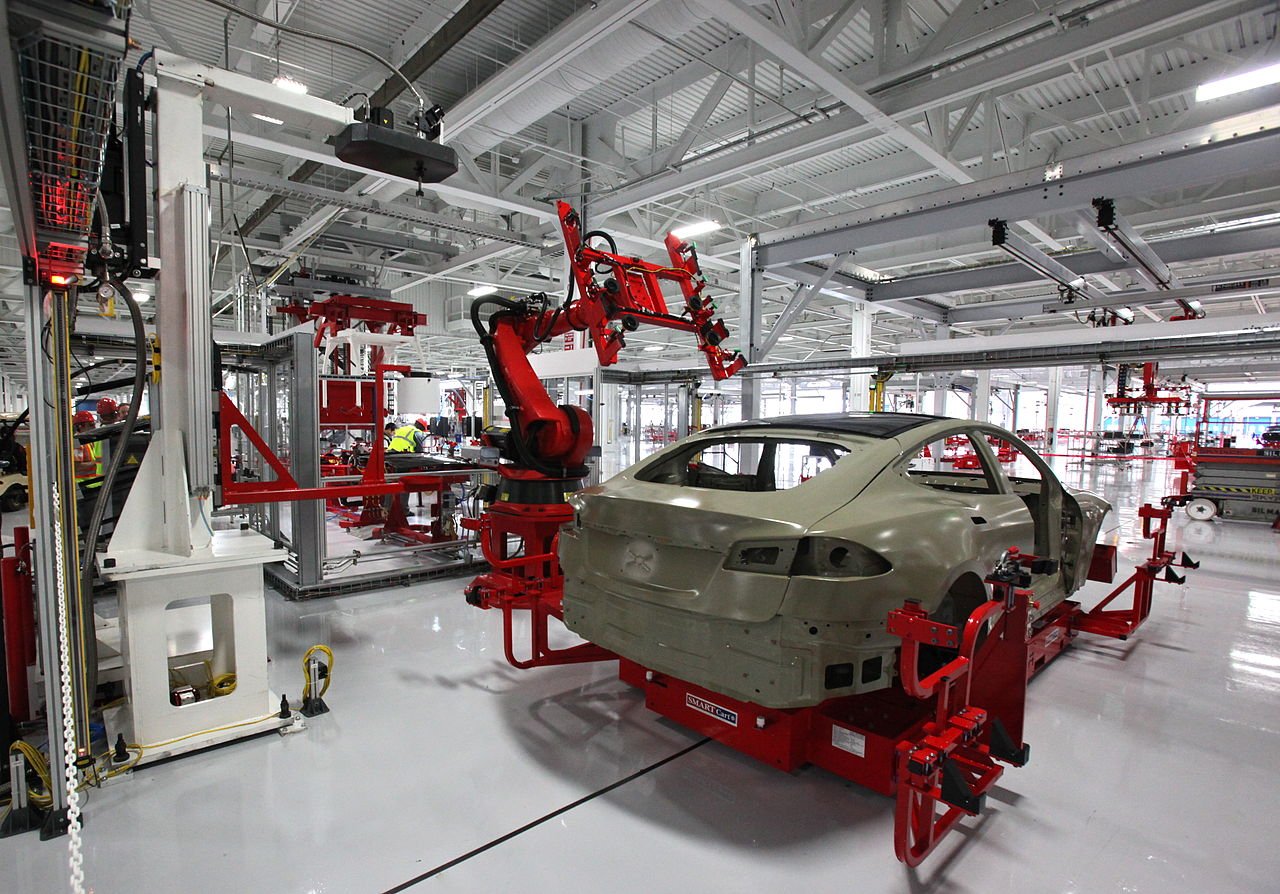
\includegraphics[height=6cm]{../pics/floss/1280px-Tesla_auto_bots}
		\caption{Tesla promises not to enforce patents (\cite{teslapatentstmt}) --credit: Steve Jurvetson}
		% https://commons.wikimedia.org/wiki/File:Tesla_auto_bots.jpg
	\end{figure}
}

\frame{
%	\frametitle{Free Software and Open Source Software}
	\frametitle{Building complex large-scale software systems (fast)}
%	\framesubtitle{An introduction to Free/Libre Open Source Software (\href{https://www.youtube.com/watch?v=Tyd0FO0tko8}{Intel, 2014})}
	\framesubtitle{An introduction to Free/Libre Open Source Software (\cite{intel2014:FLOSS})}
	\begin{figure}
	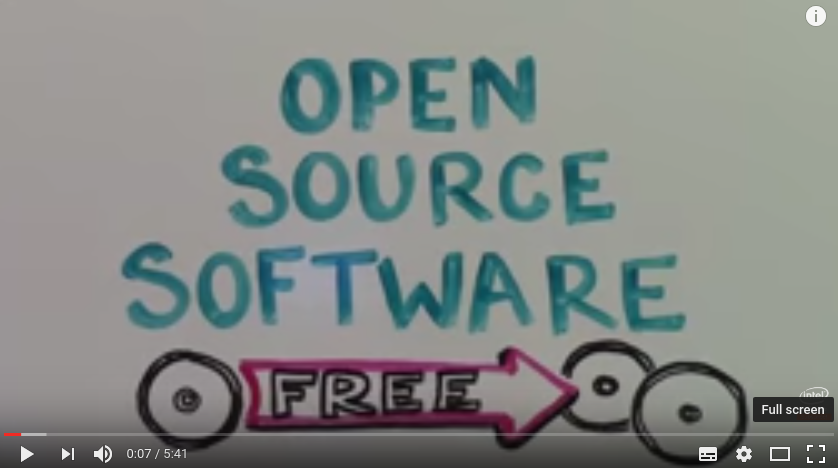
\includegraphics[height=5cm]{../pics/intel-FLOSS-intro}
	\caption{\url{https://www.youtube.com/watch?v=Tyd0FO0tko8}}
	\end{figure}
	\tiny \copyright \href{https://www.youtube.com/watch?v=Tyd0FO0tko8}{Intel Software (2014)}
}

\frame{
	\frametitle{Blockchain is Open/Free by design}
	\begin{figure}
	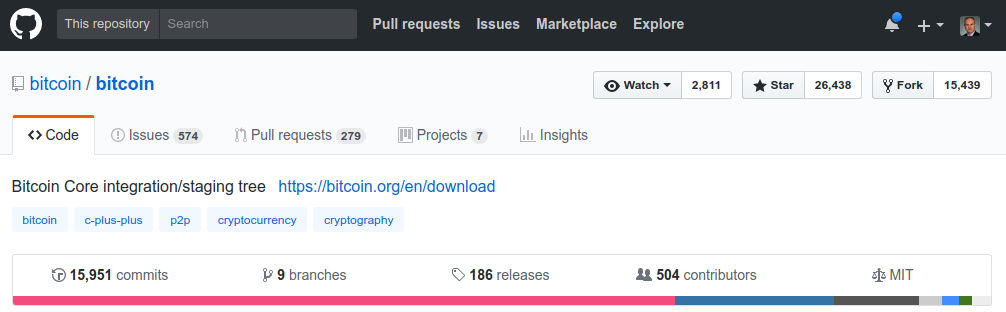
\includegraphics[width=10cm]{../../pics/bitcoin-core-github}
	%
\includegraphics[width=8cm,left]{../../pics/bitcoin-core-github-license}
	
\includegraphics[width=10cm]{../../pics/bitcoin-core-github-license}
	\end{figure}
}

\frame{
	\frametitle{Intellectual Property Rights (and constraints)}
	\begin{itemize}
		\item Copyright
		\item Patents
		\item Trademark
		\item Trade Secrets
	\end{itemize}
}

\begin{frame}   % the four freedoms
	\frametitle{Free Software}
	\begin{figure}
		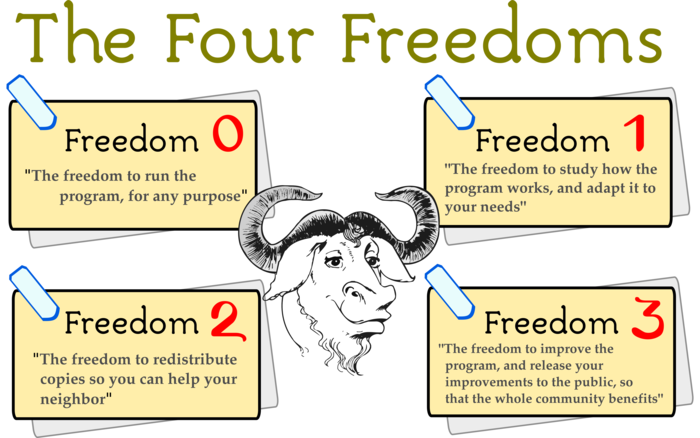
\includegraphics[width=11cm]{../pics/scaled_full_00c40105cea4c0aa3e9f}
	\end{figure}
\end{frame}


% ======================================================================================================
%                                     What is Blockchain and what does it help?
% ======================================================================================================
\section{Introducing Blockchain}
\subsection{What is Blockchain?}
\frame{
	\frametitle{Decentralization}
	\begin{figure}
		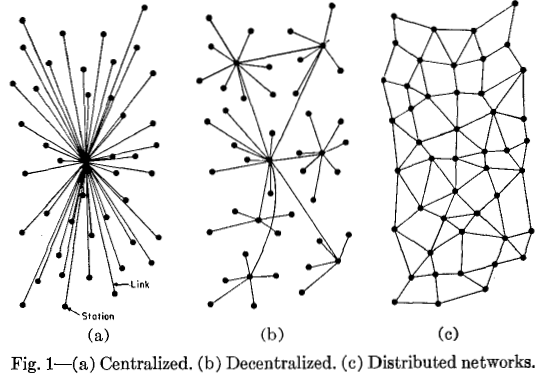
\includegraphics[height=6cm]{../pics/ethereum/networktypes}
	\end{figure}
}

\frame{
	\frametitle{What is Blockchain?}
	\begin{figure}
		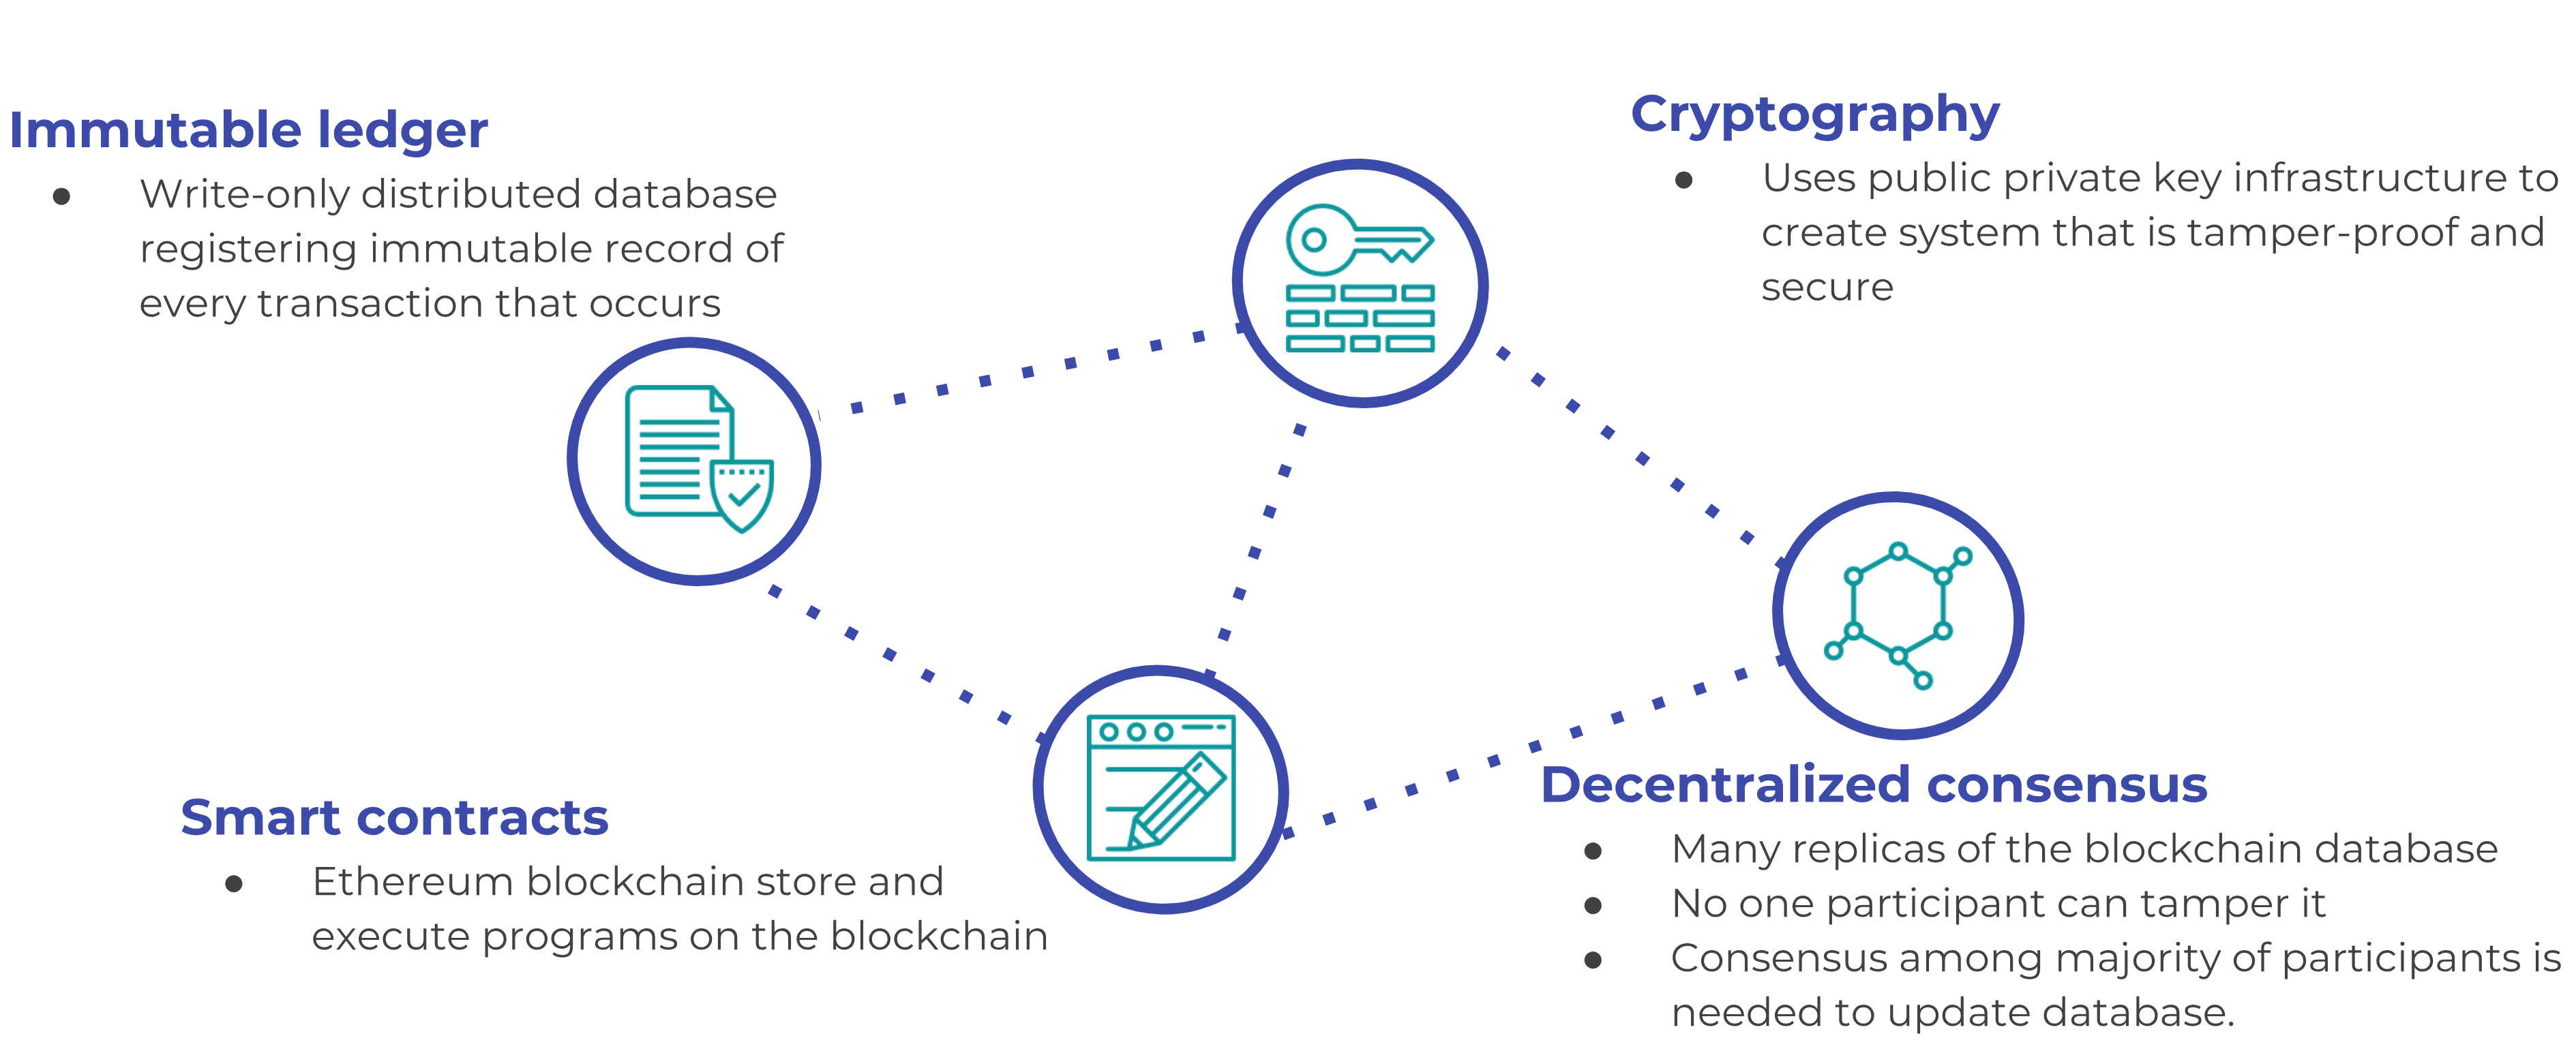
\includegraphics[width=11cm]{../pics/ConsenSys/what_is_blockchain}
	\end{figure}
}

\frame{
	\frametitle{Cryptographic Primitives}
	\begin{figure}
		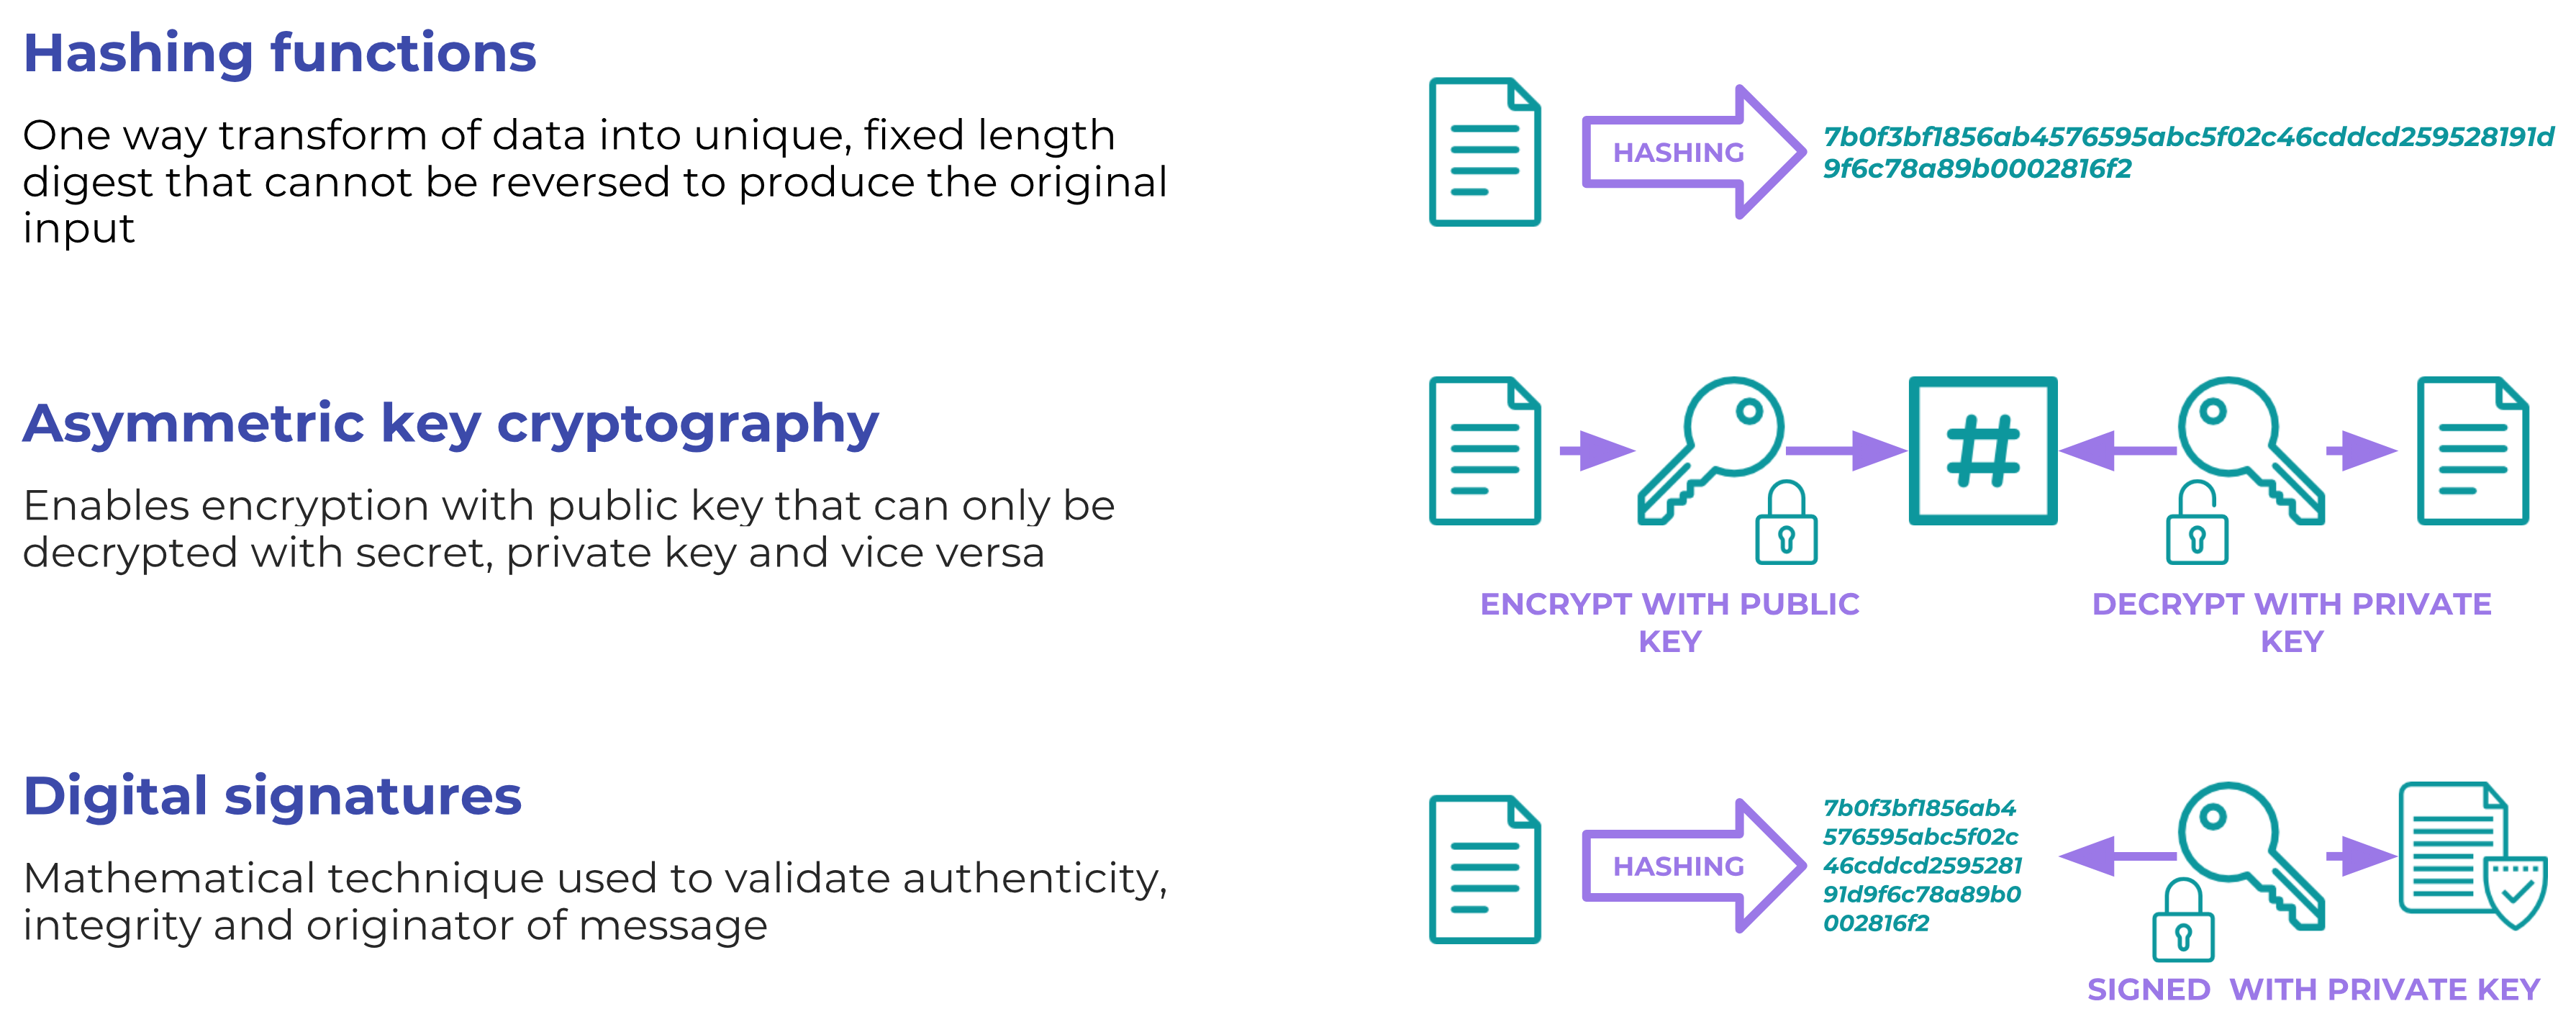
\includegraphics[width=11cm]{../pics/ConsenSys/cryptographic_primitives}
	\end{figure}
}

% --------------------------------------- Design Patterns -------------------------------------
\subsection{Design Patterns}
\frame{
	\frametitle{Token-Curated Registry Pattern}
	\begin{figure}
		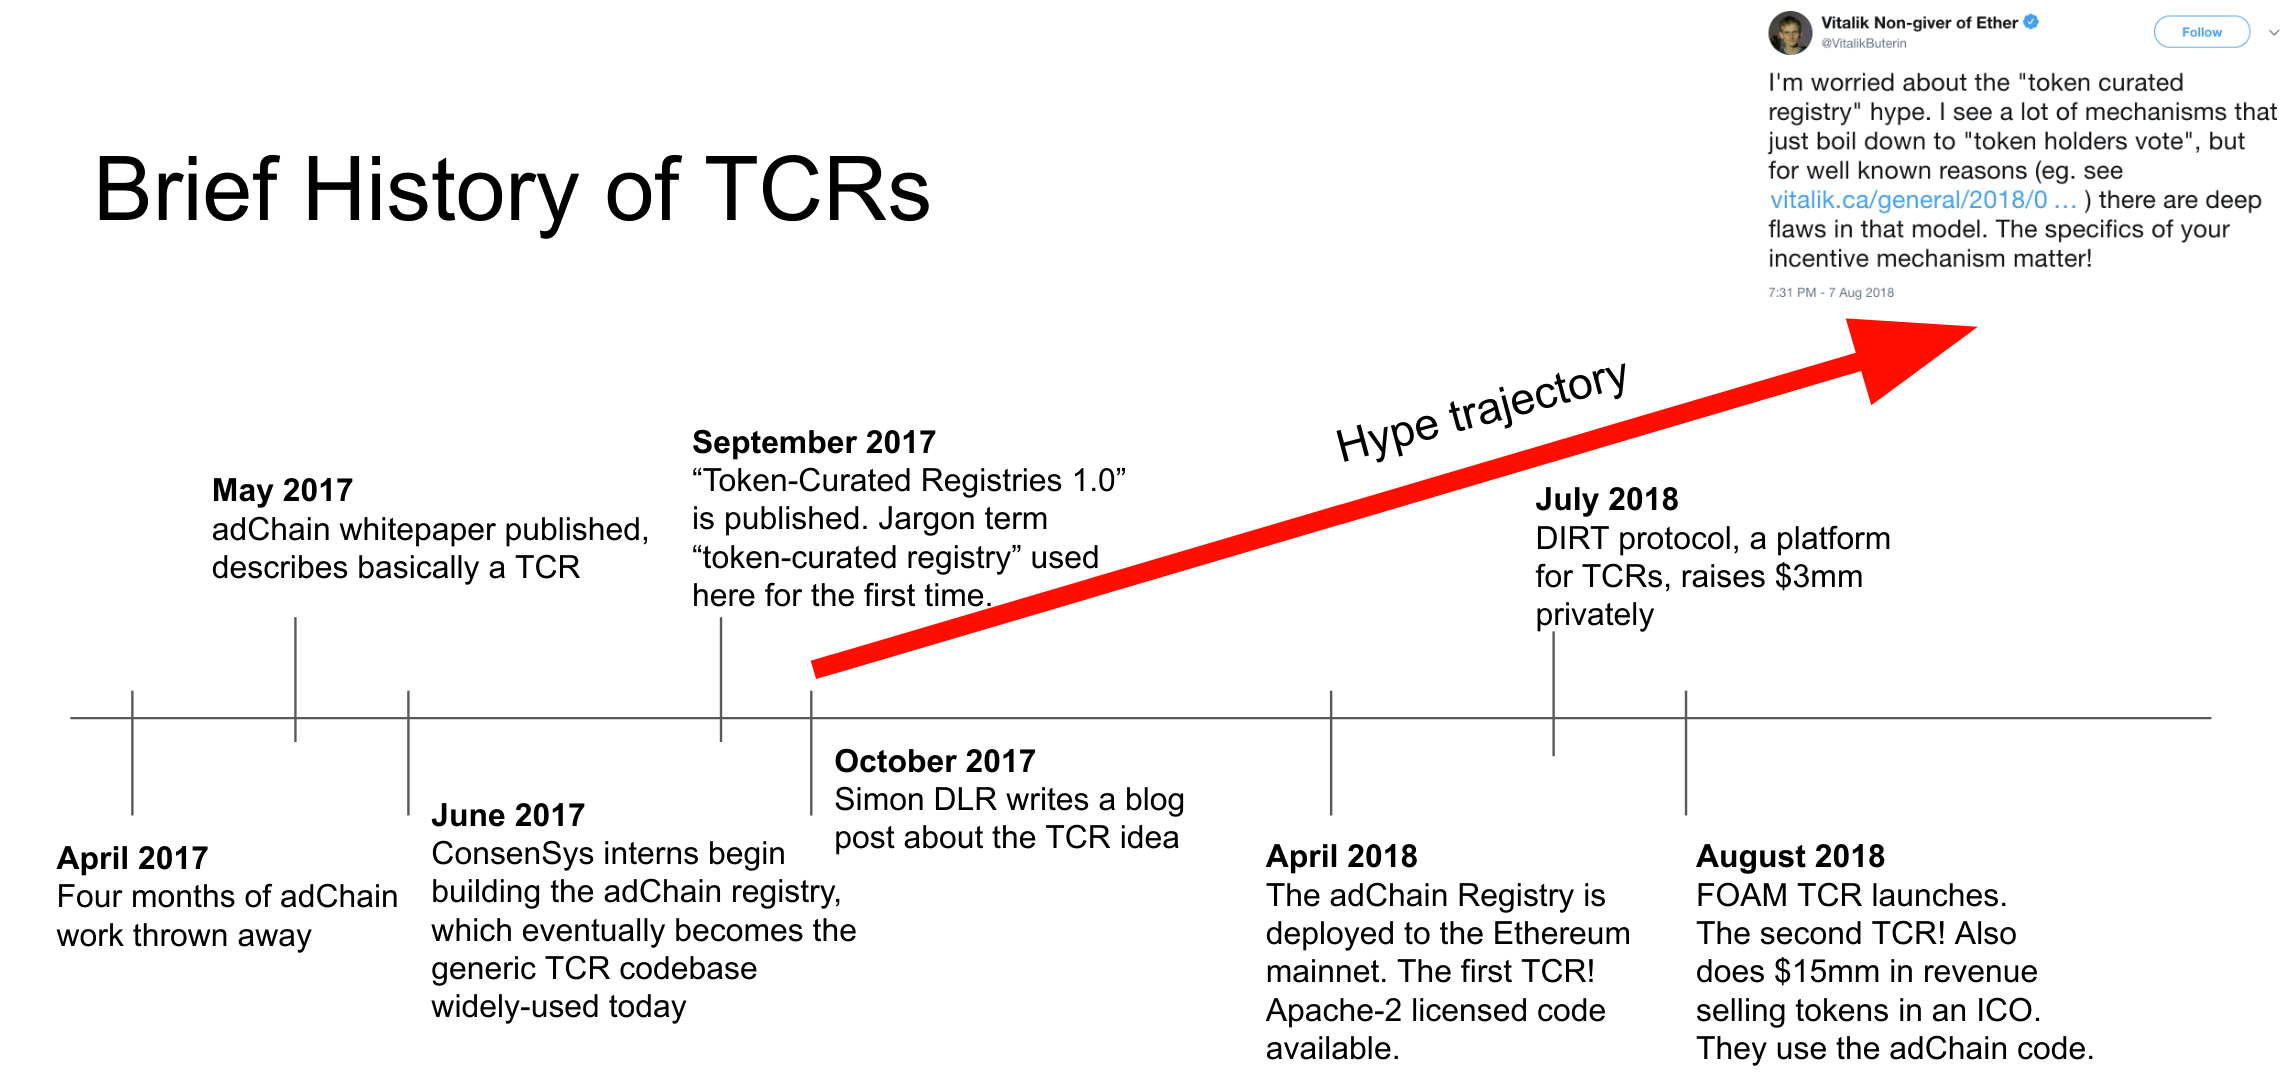
\includegraphics[width=11cm]{../pics/ConsenSys/Design_Patterns/TCR_history_2018H1}
		\caption{from Mike \citeauthor{mikegoldin2018:tcrprezi}'s presentation (\citeyear{mikegoldin2018:tcrprezi})}
	\end{figure}
}

\frame{
	\frametitle{Use Cases in Media \& Entertainment}
	\begin{figure}
		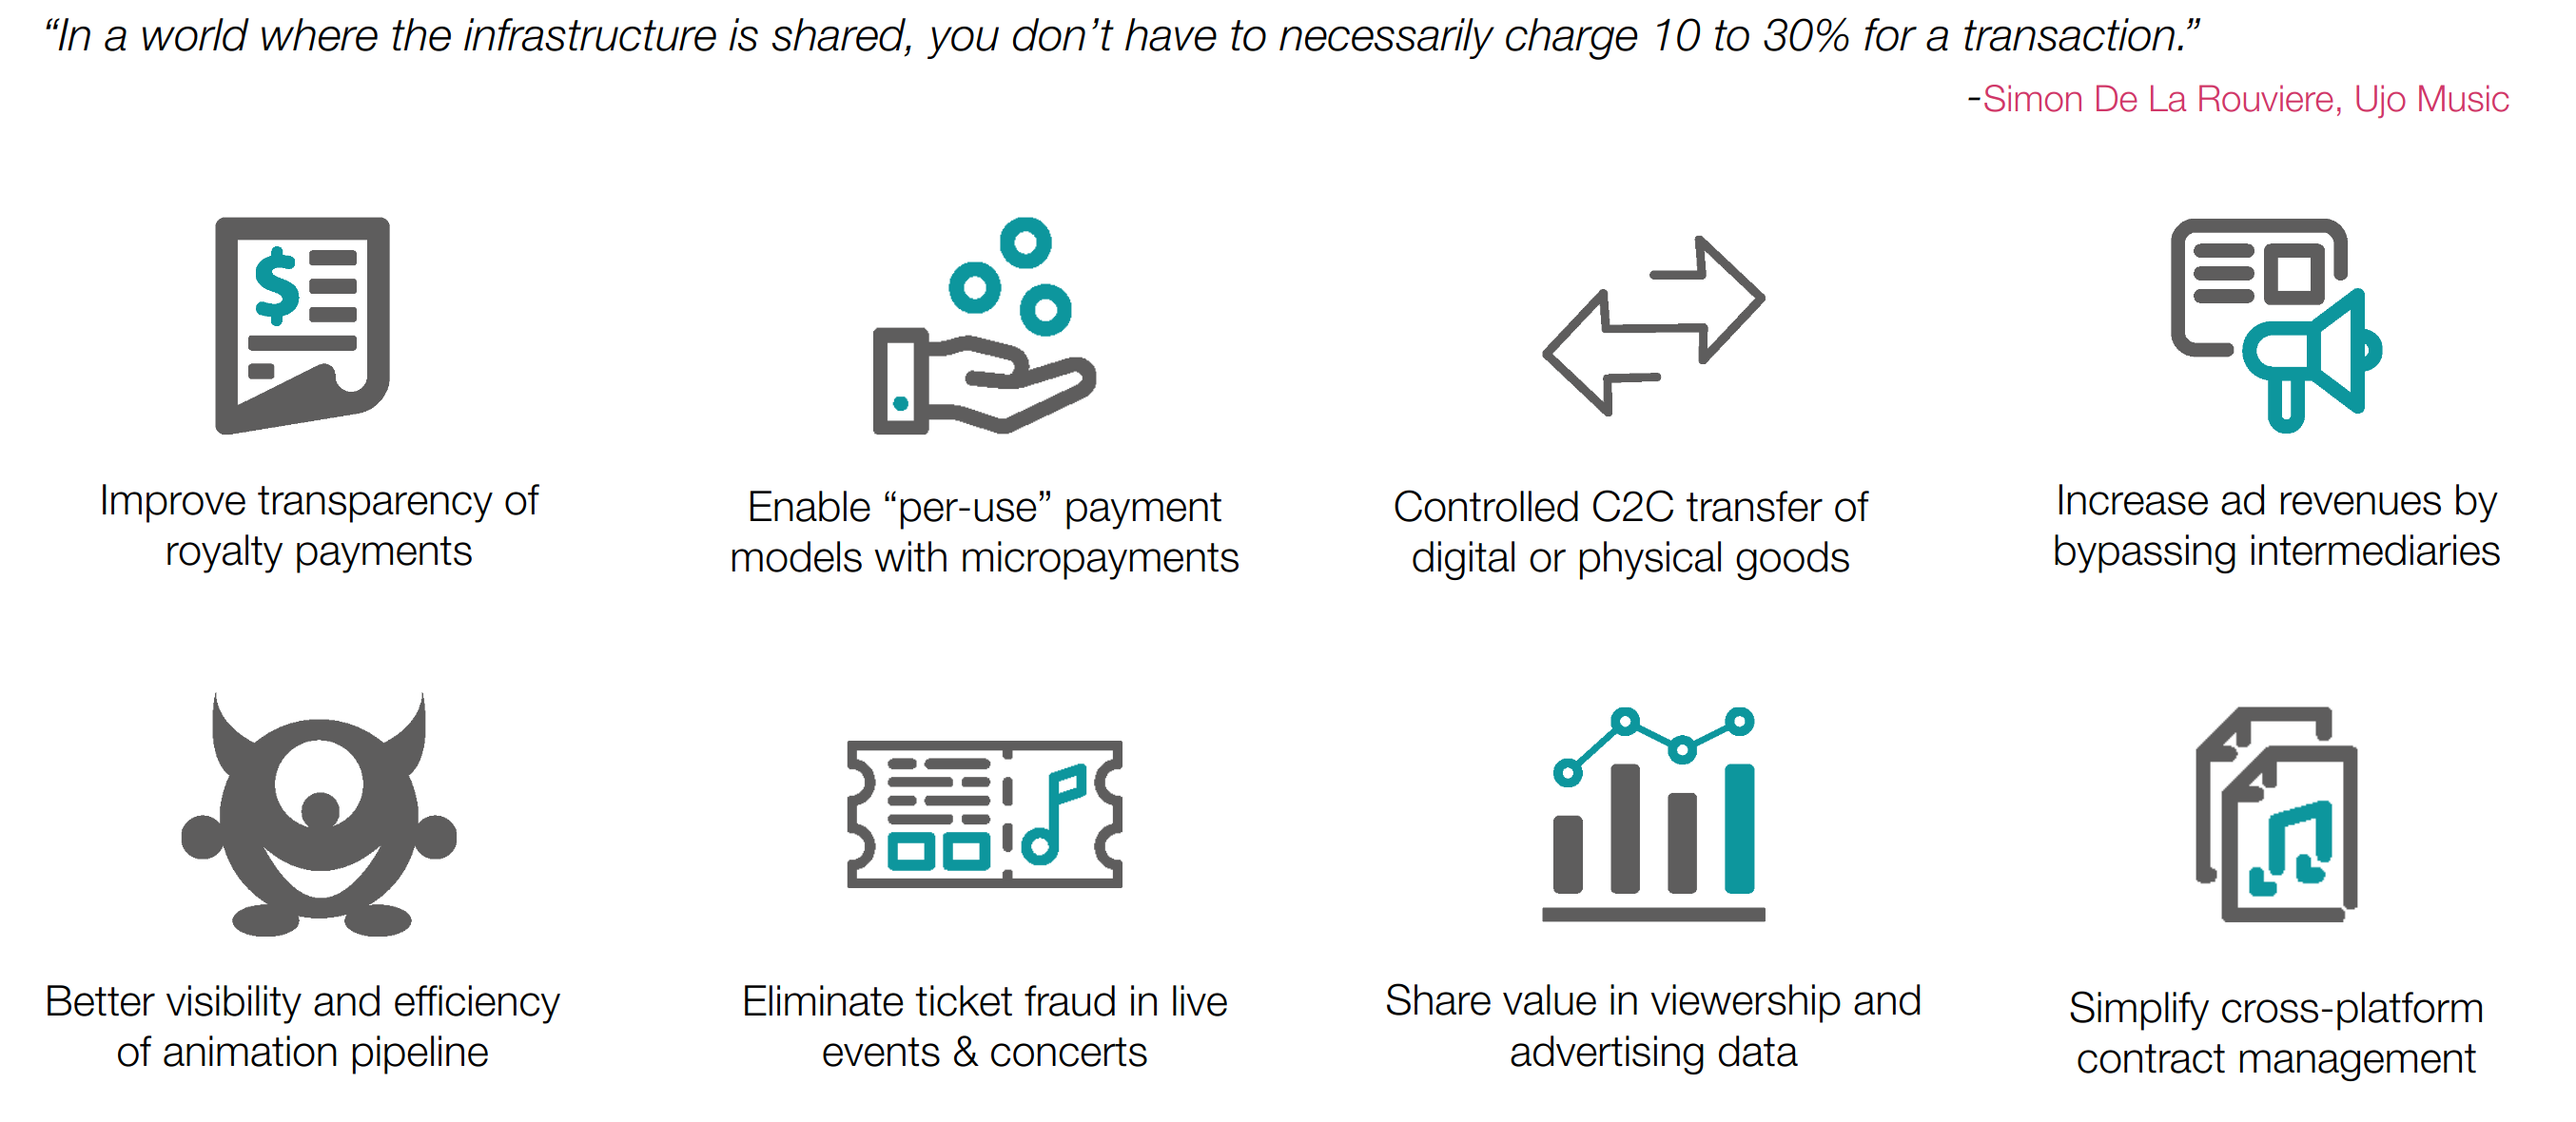
\includegraphics[width=11cm]{../pics/ConsenSys/industry/use-case-ME}
	\end{figure}
}

% ======================================================================================================
%                                     Case studies -- a few examples of blockchain use for IP
% ======================================================================================================
\section{Case studies}

\begin{frame}   
	\frametitle{Case study: Berntein}
	\begin{figure}
		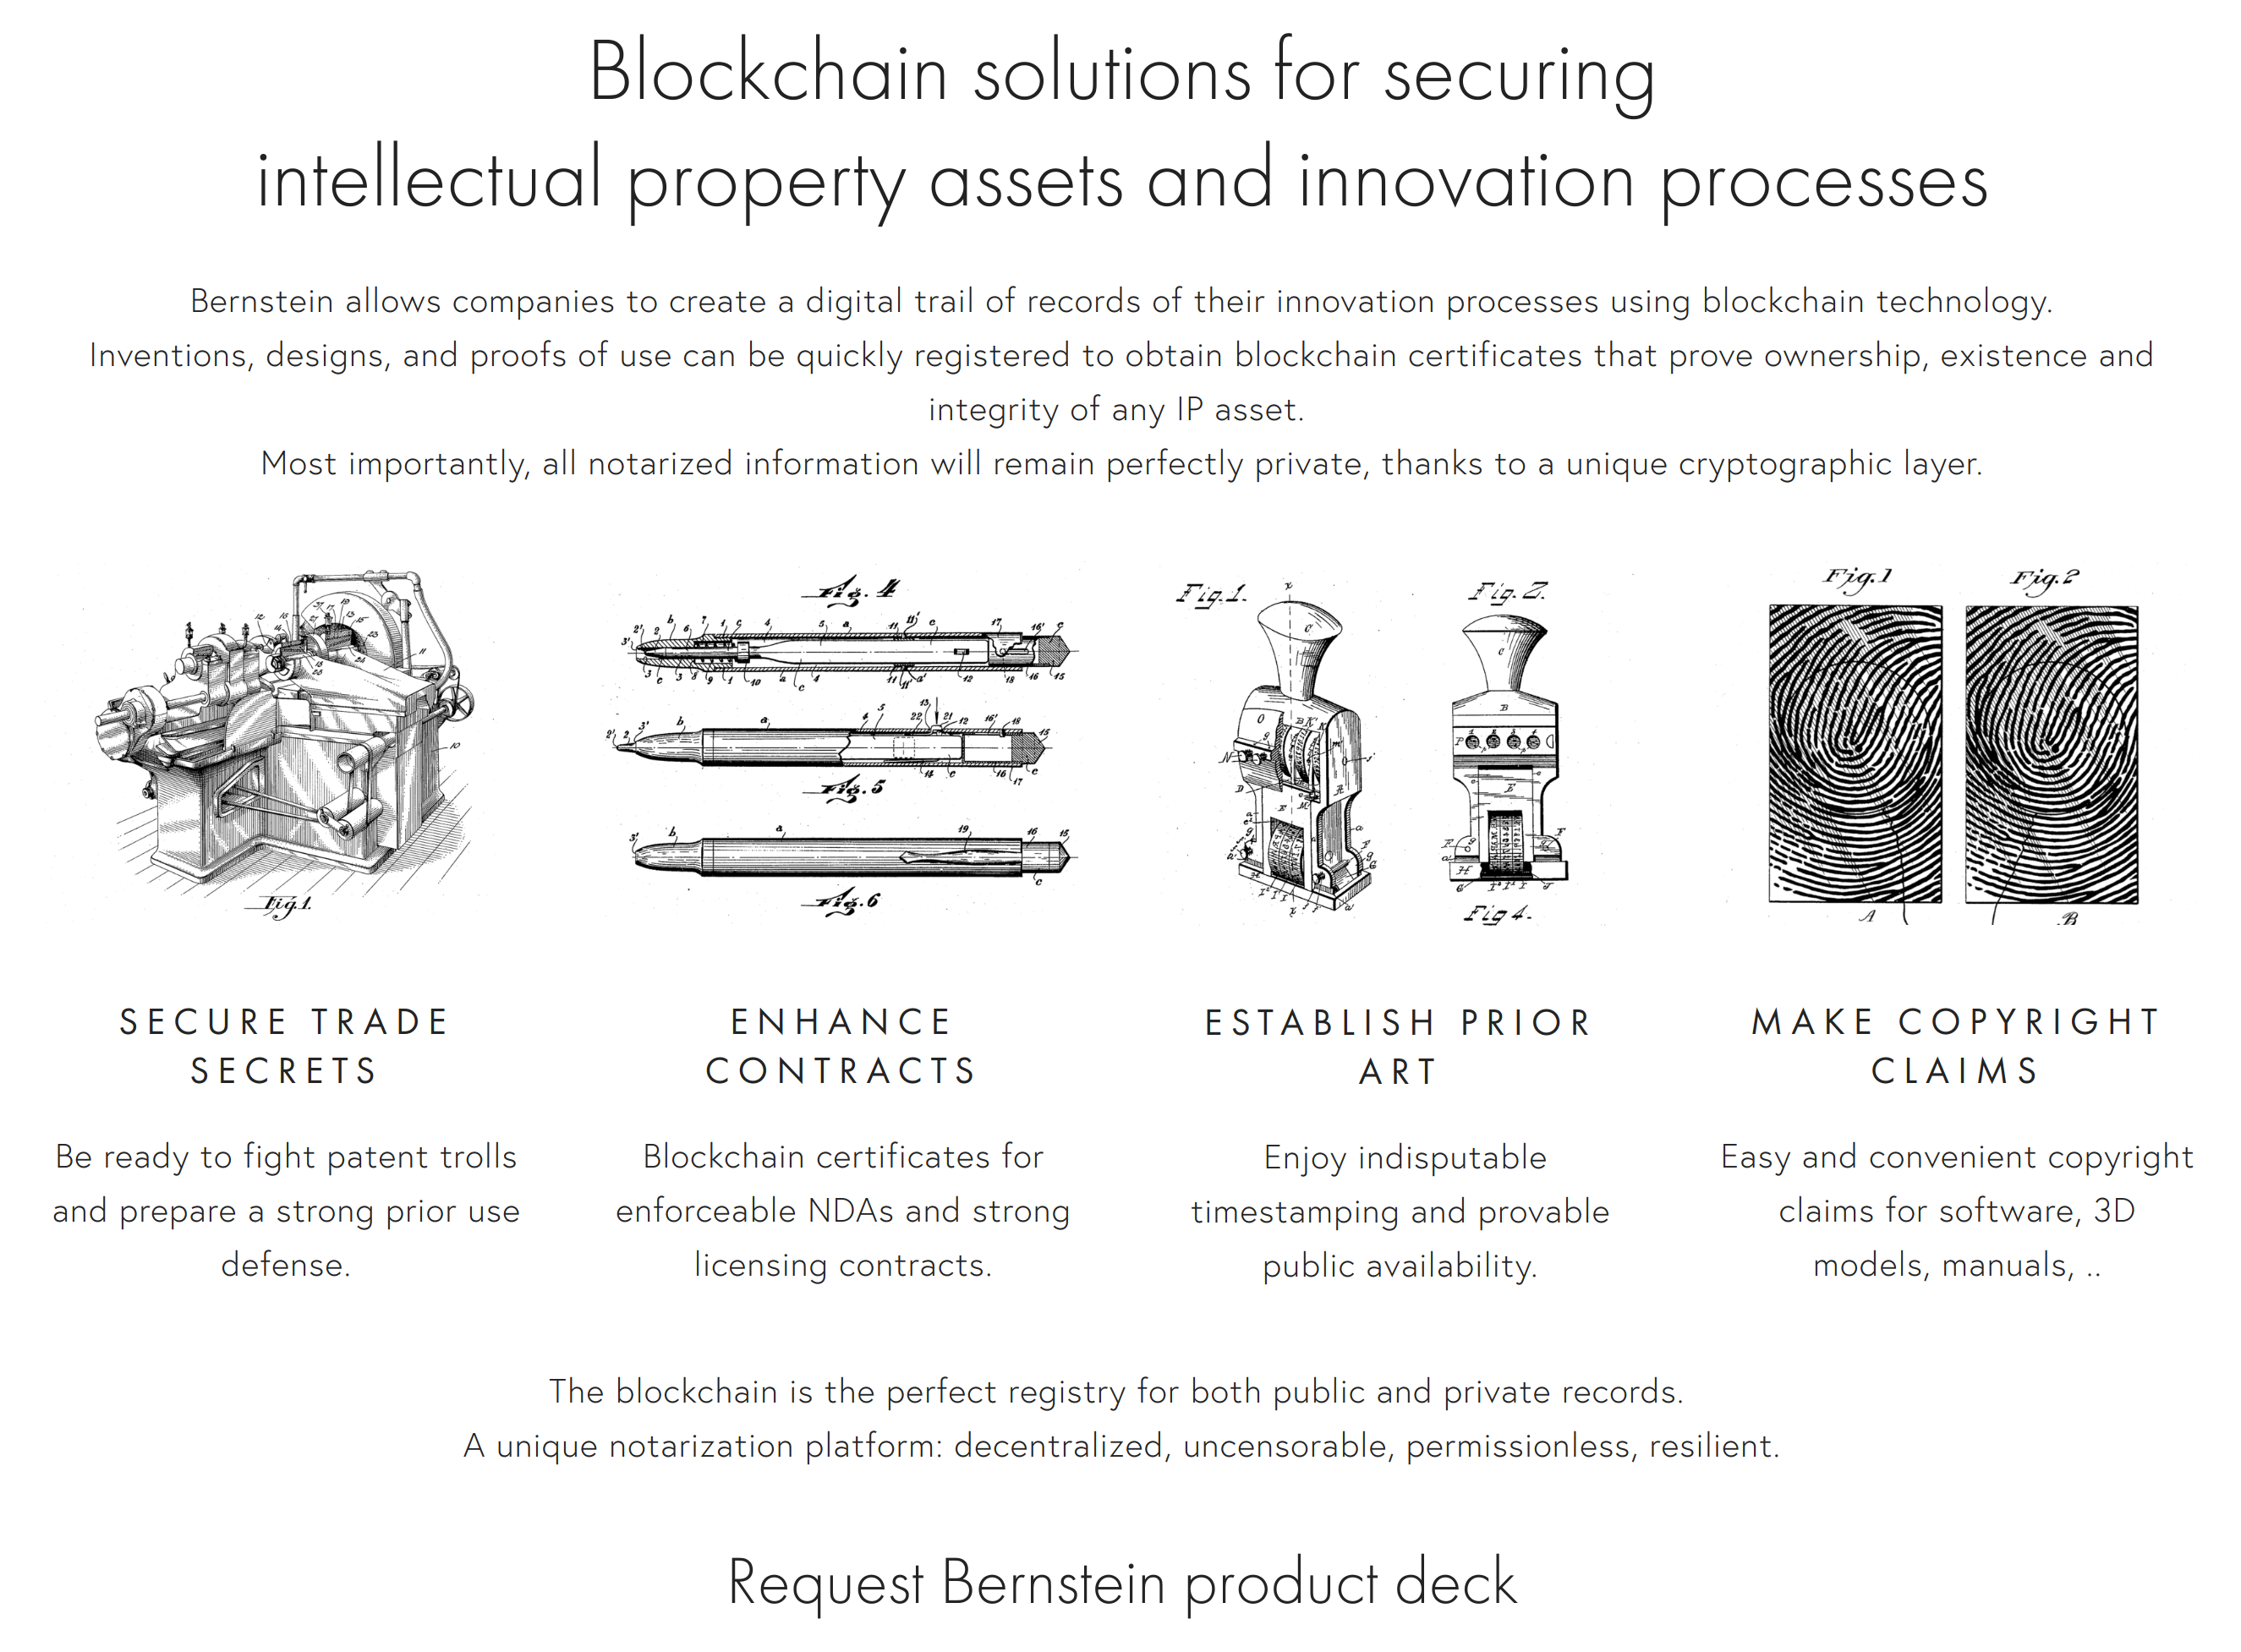
\includegraphics[width=10cm]{../pics/case_studies/bernstein}
		\caption{\url{https://www.bernstein.io}}
	\end{figure}
\end{frame}

\begin{frame}   
	\frametitle{Case study: Vaultitude}
	\begin{figure}
		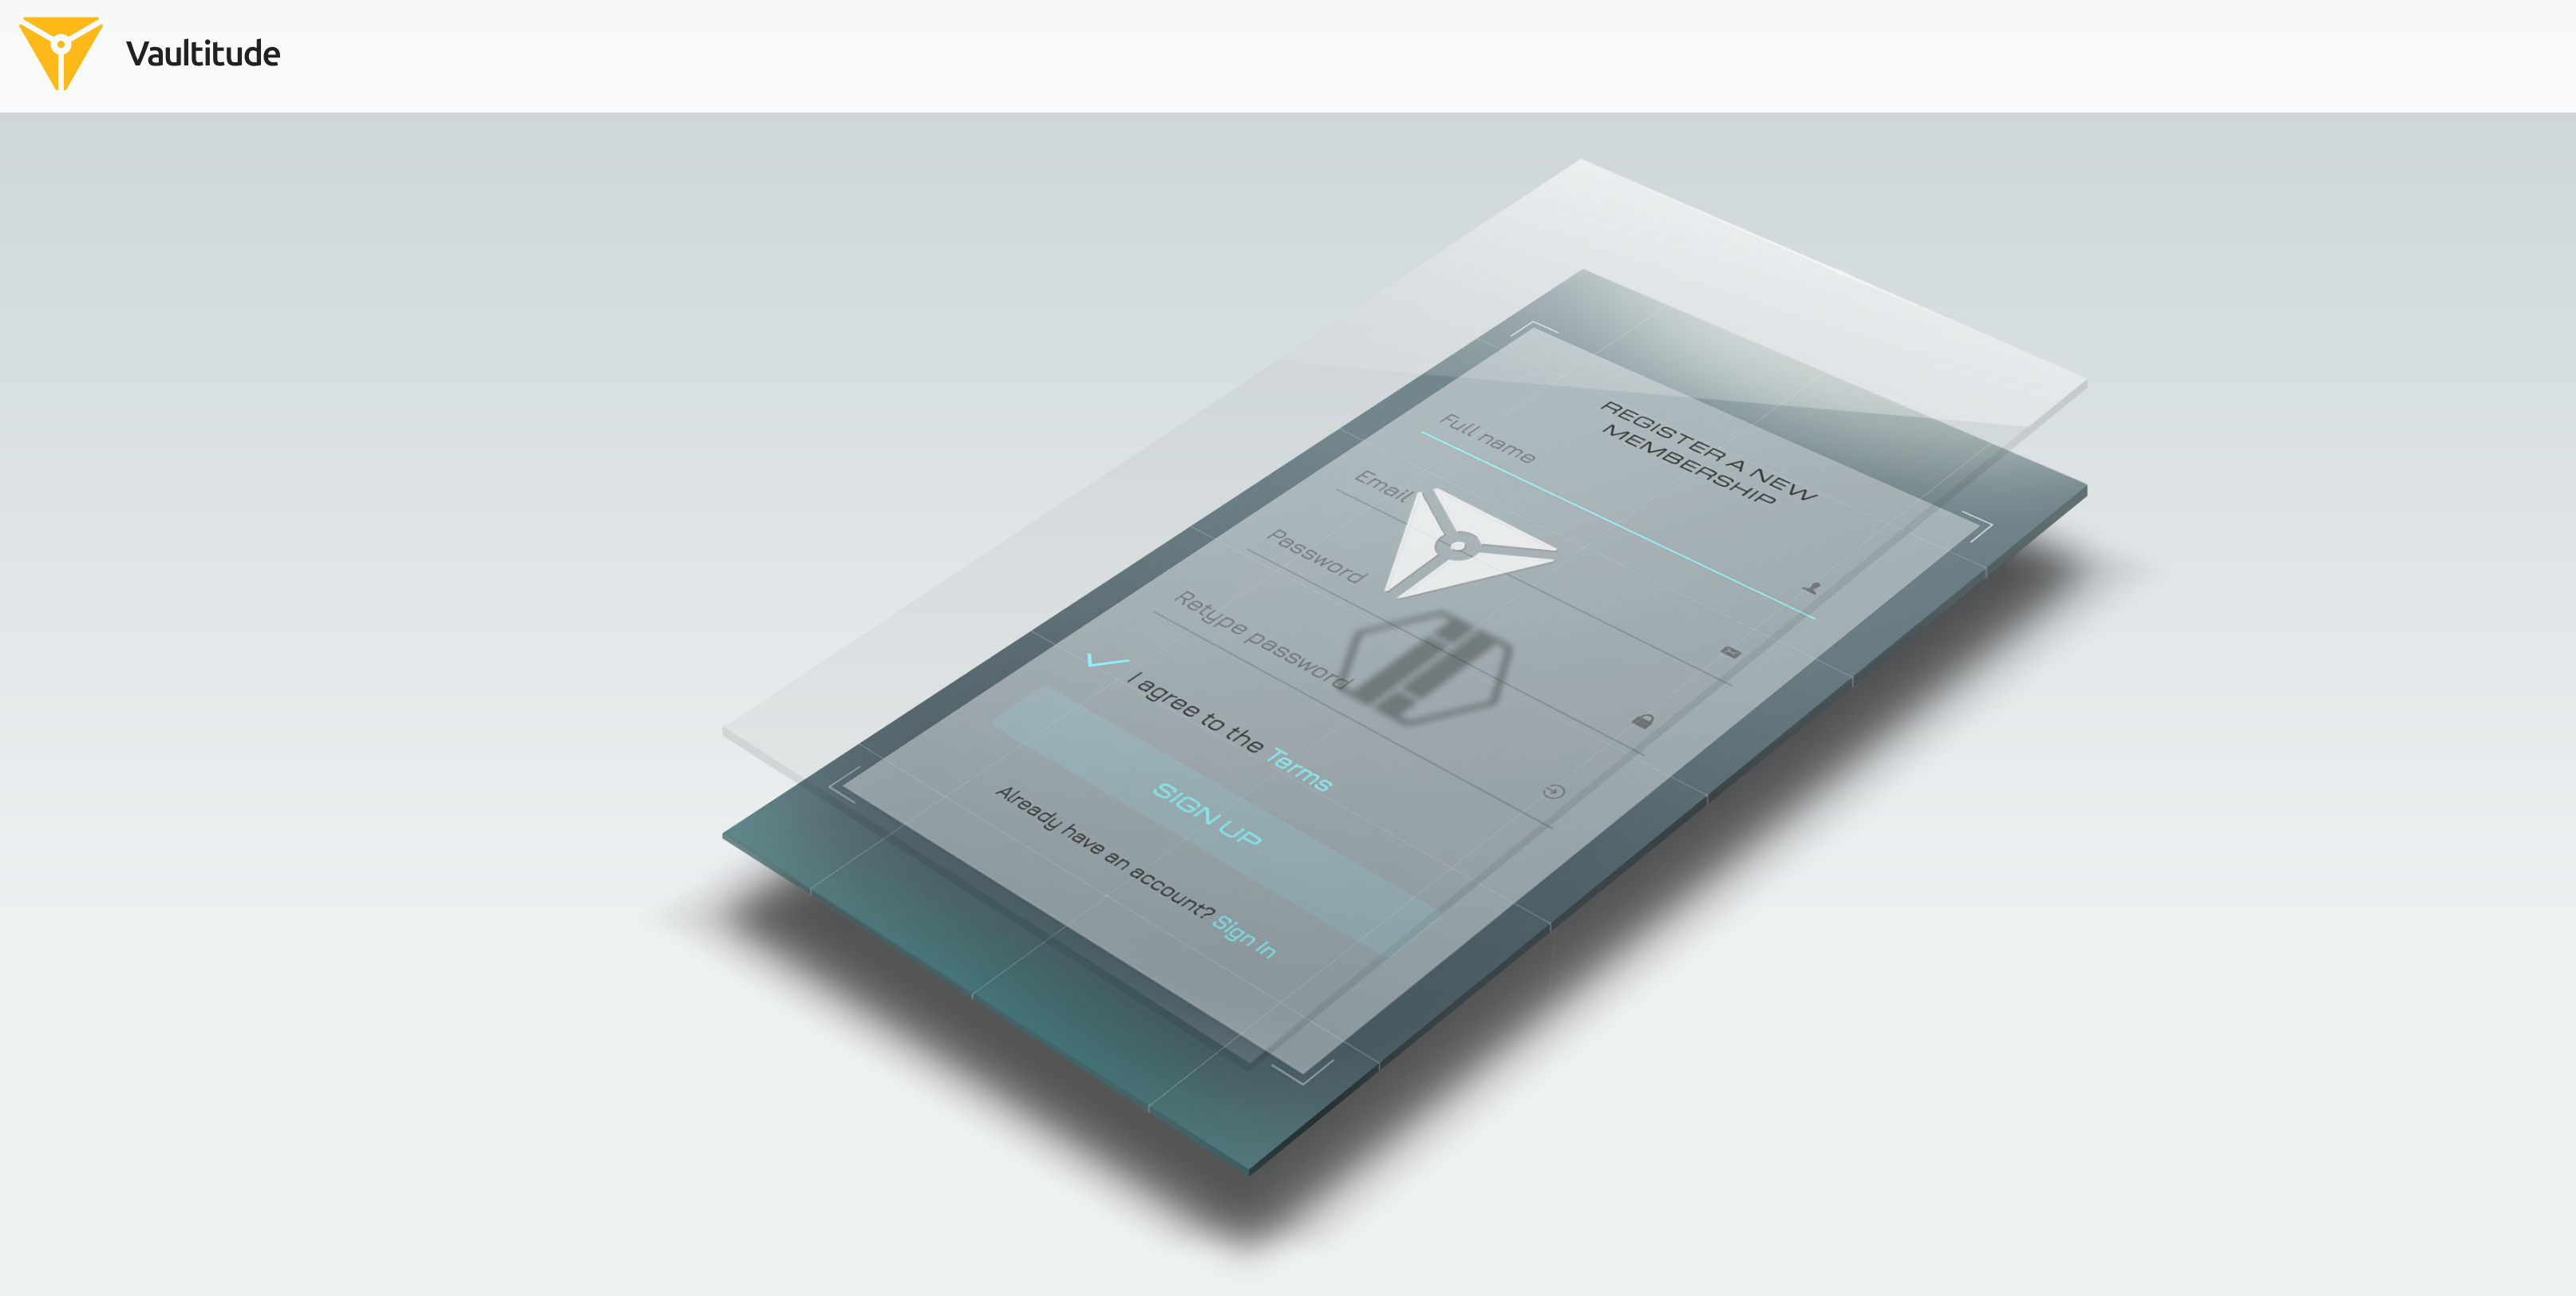
\includegraphics[width=11cm]{../pics/case_studies/vaultitude}
		\caption{\url{https://vaultitude.com}}
	\end{figure}
\end{frame}

\begin{frame}   
	\frametitle{Case study: Baoquan}
	\begin{figure}
		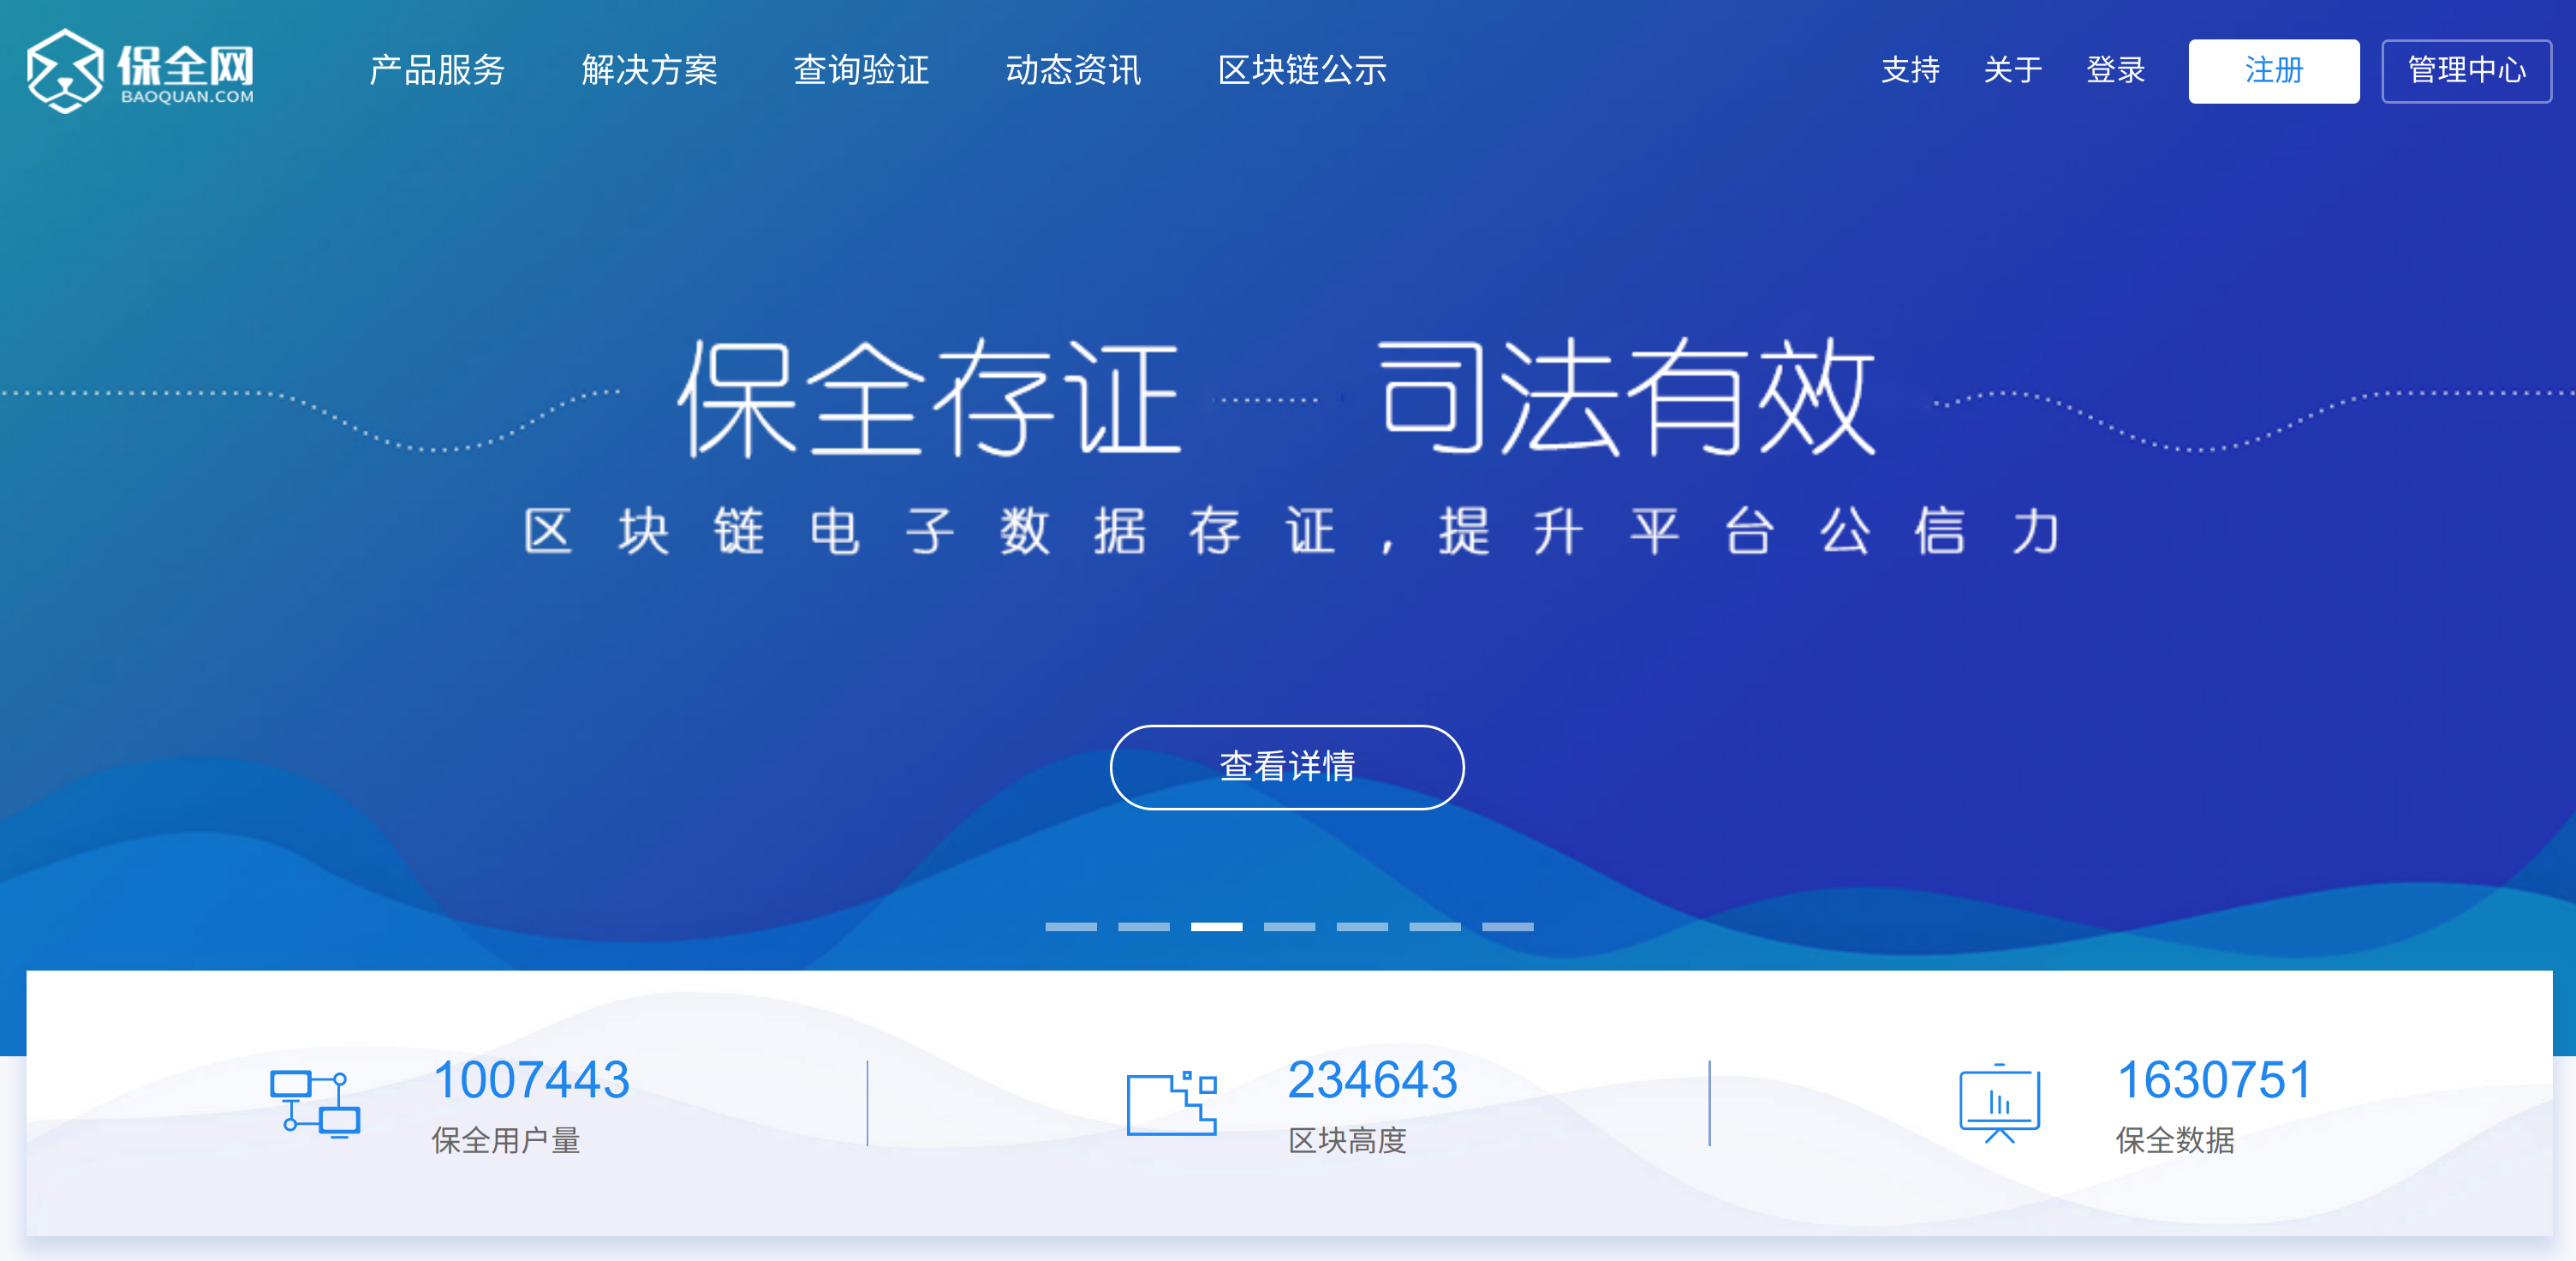
\includegraphics[width=11cm]{../pics/case_studies/baoquan}
		\caption{The Hangzhou Internet Court accepted evidence from the Baoquan Blockchain on a copyright case (\cite{chinesecourt2018})}
	\end{figure}
\end{frame}

\frame{
	\frametitle{Case study: Viant}
	\framesubtitle{Tracking IP (and other) Assets}
	\begin{figure}
		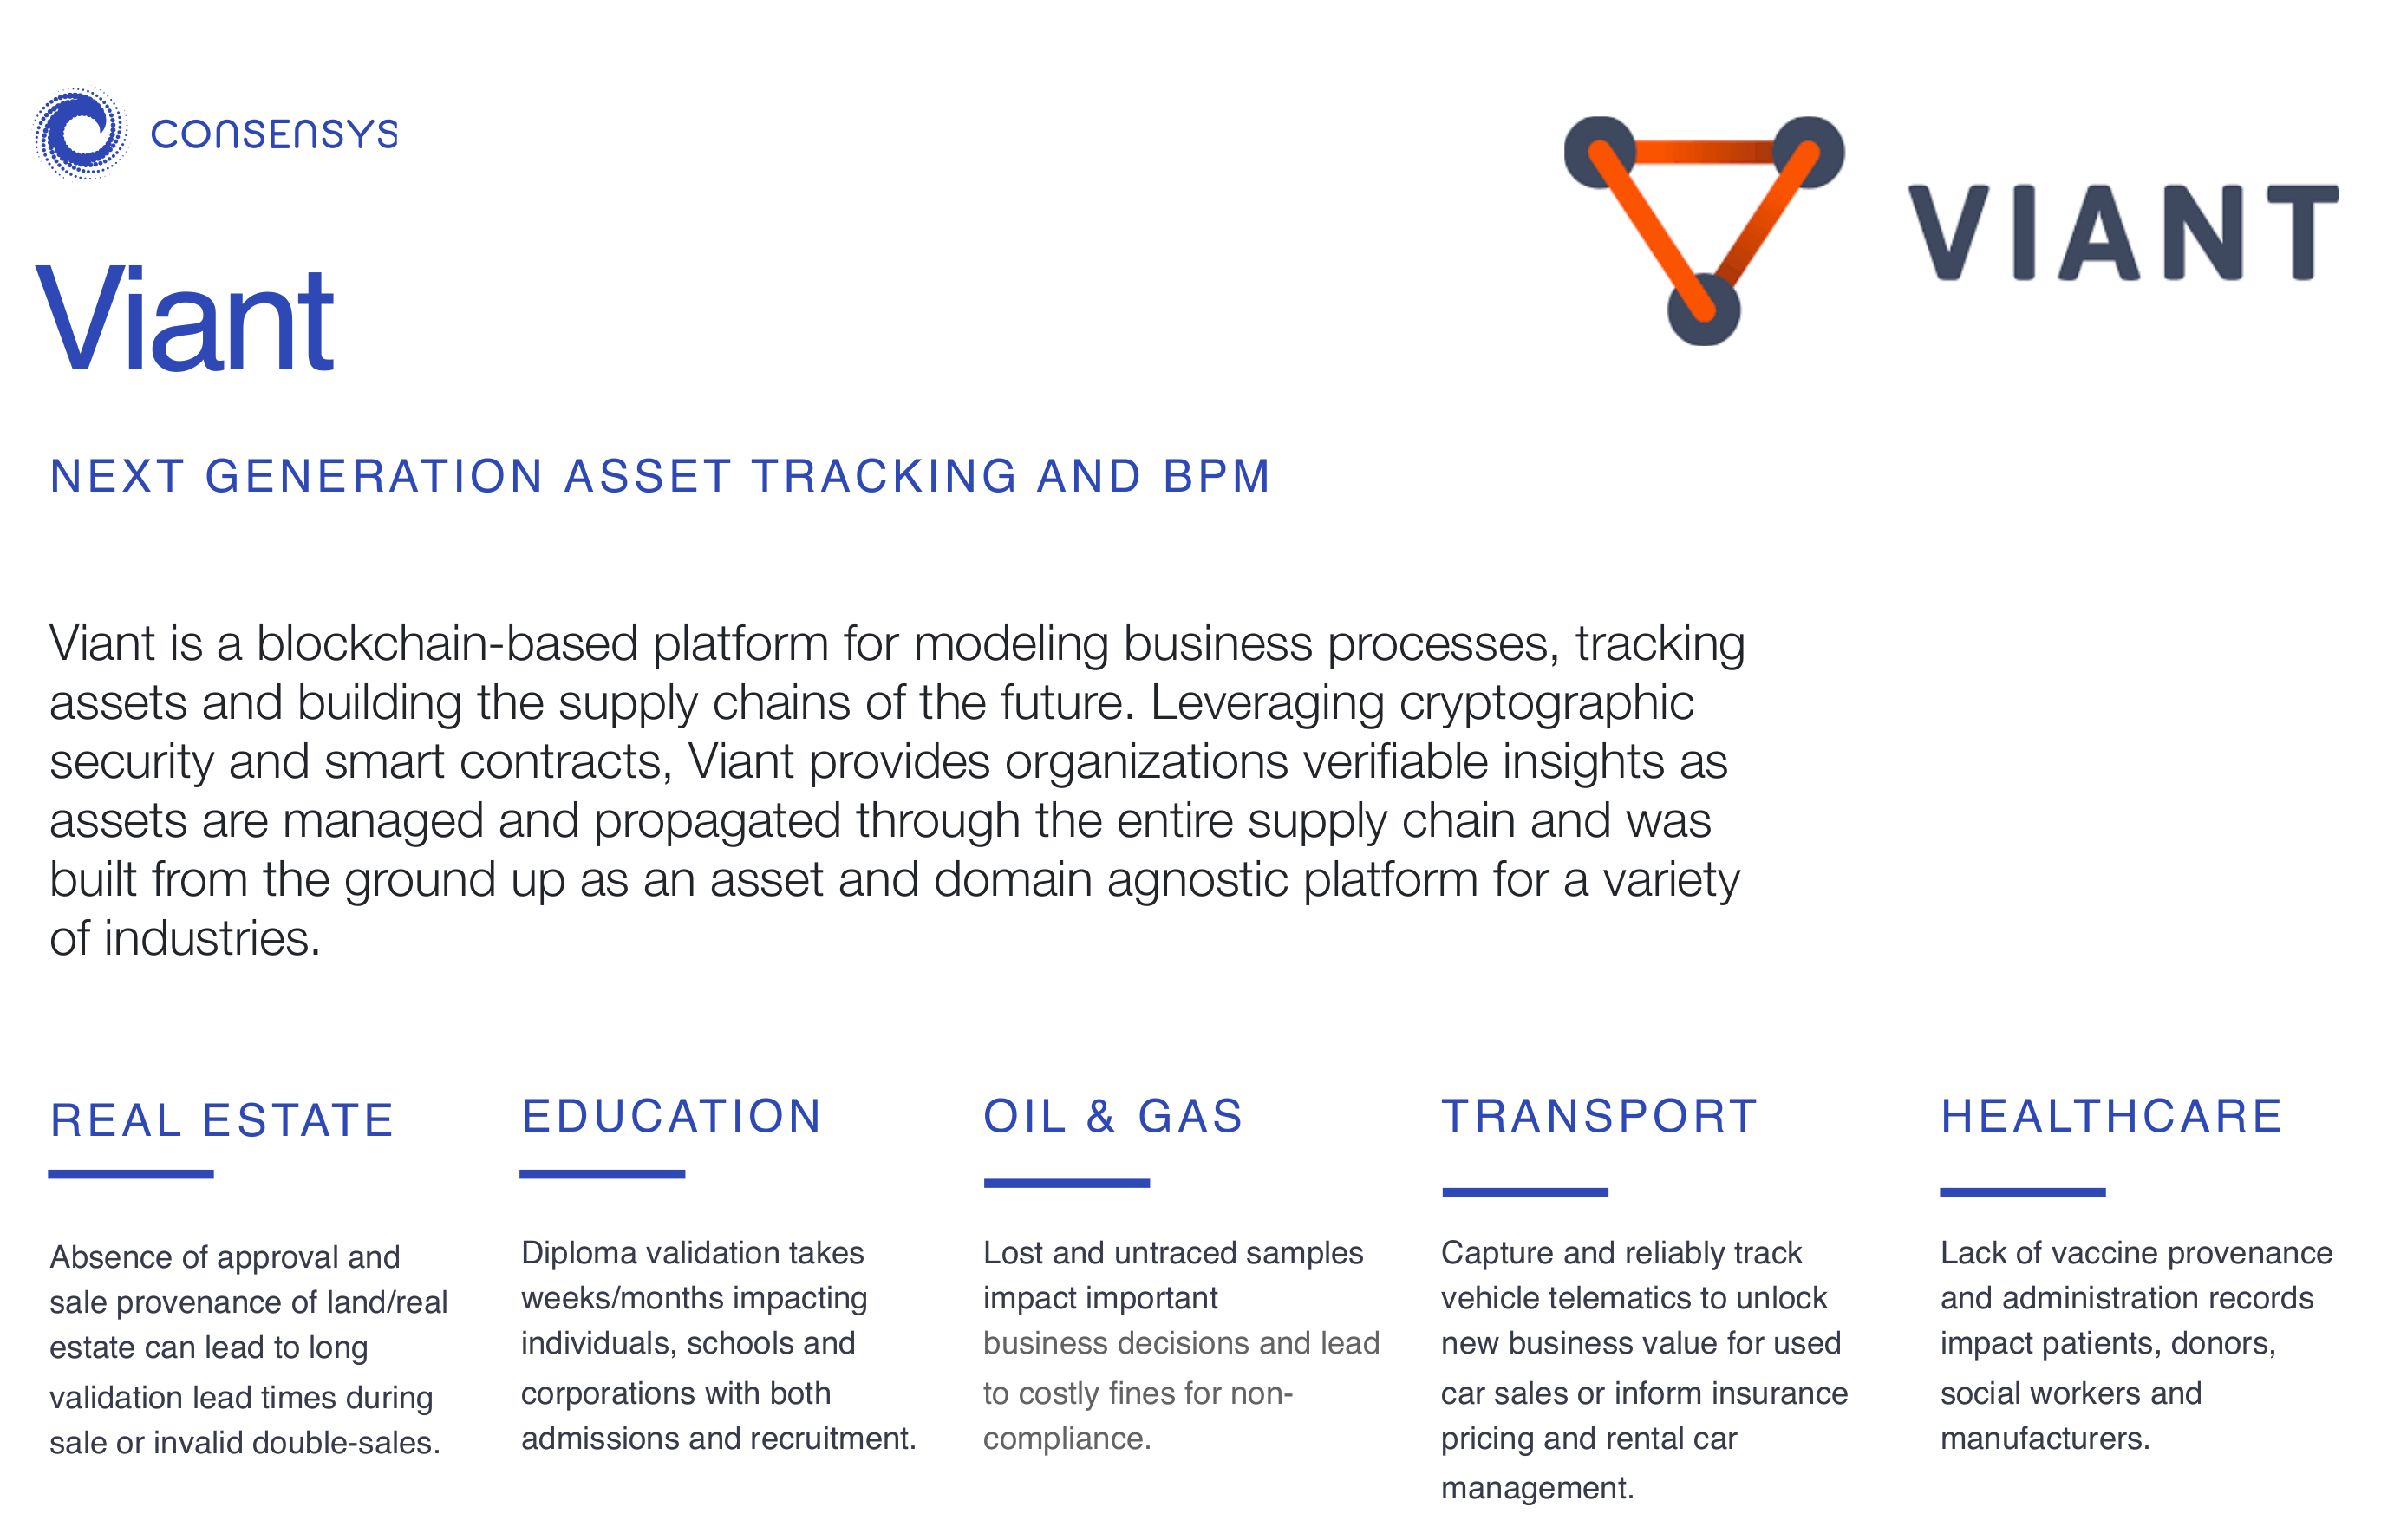
\includegraphics[width=11cm]{../pics/ConsenSys/spokes/viant-top}
		\caption{\url{https://viant.io}}
	\end{figure}
}

\frame{
	\frametitle{Complementary tools: Alethio}
	\framesubtitle{Big Data and Analytics on Ethereum}
	\begin{figure}
		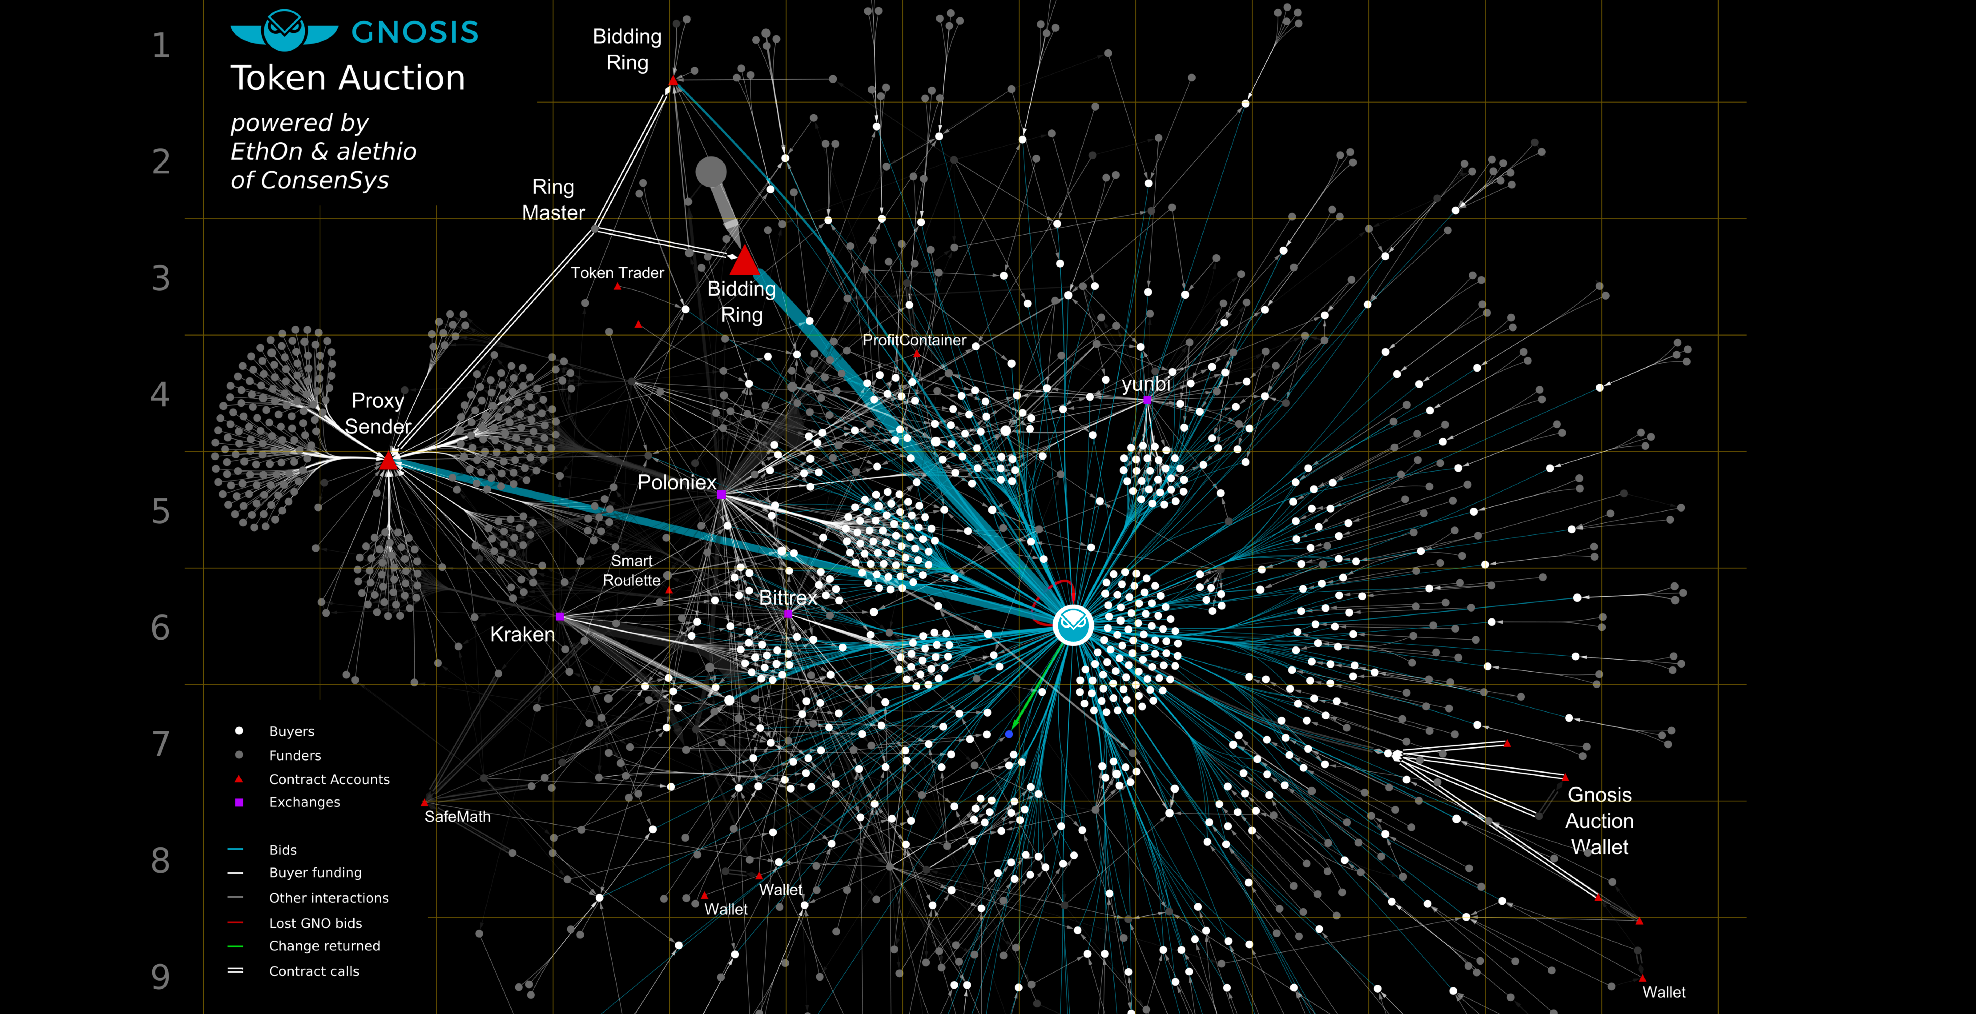
\includegraphics[width=11cm]{../pics/ConsenSys/alethio-tracking-viz}
		\caption{\url{https://aleth.io}}
	\end{figure}
}

\frame{
	\frametitle{Developer-friendly marketplace: The Bounties Network}
	\framesubtitle{Why not getting paid for your work?}
	\begin{figure}
		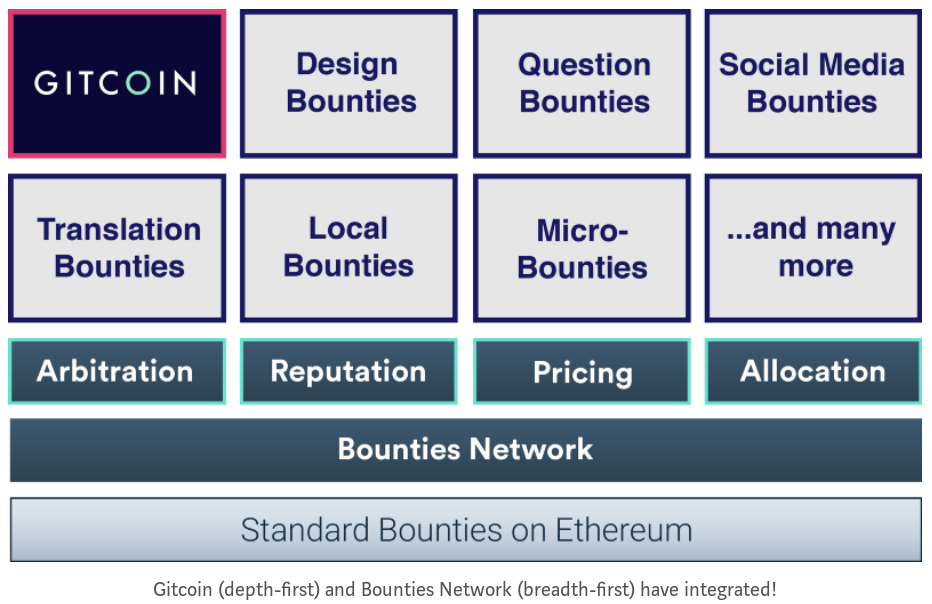
\includegraphics[width=11cm]{../pics/ConsenSys/bounties_network_stack}
		\framesubtitle{\url{https://bounties.network}}
	\end{figure}
}

\frame{
	\frametitle{Gitcoin}
	\framesubtitle{Gitcoin is not a coin}
	\begin{figure}
		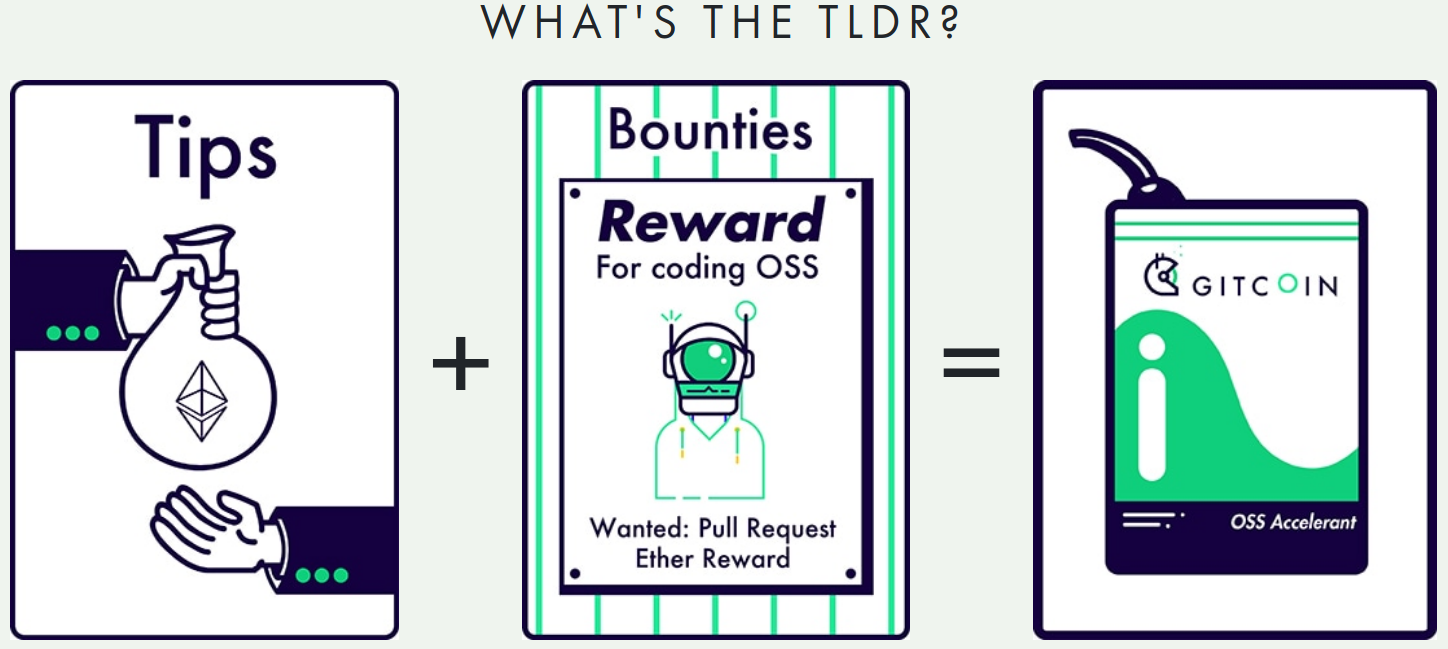
\includegraphics[width=11cm]{../pics/ConsenSys/gitcoin-tldr}
		\caption{\url{https://gitcoin.co}}
	\end{figure}
}

